\documentclass[runningheads]{llncs}
\usepackage[english]{babel}
\usepackage[T1]{fontenc}
\usepackage[utf8]{inputenc}
\let\proof\relax
\let\endproof\relax
\usepackage{iftex}
\usepackage[dvipdfm]{graphicx}
\usepackage{rotating}
\usepackage{bmpsize}
\usepackage{wrapfig}
\usepackage{lscape}
\usepackage{rotating}
\usepackage{listings}
\usepackage{amsmath}
\usepackage{amssymb}
\usepackage{mathtools}
\usepackage{amsfonts}
\usepackage{hyperref}
\usepackage{array}
\usepackage{booktabs}
\usepackage{multicol}
\usepackage{biblatex}
\usepackage[version=4]{mhchem}
\usepackage{siunitx}
\usepackage{longtable,tabularx}
\usepackage{times}
\usepackage{subcaption}
\usepackage{xcolor}
\usepackage{multirow}
\usepackage{enumitem}
\usepackage{calc}

\newlength{\tabwidth}
\newlength{\tabwidthi}
\newlength{\tabwidthii}
\newlength{\tabwidthiii}
\newcommand{\tabsize}{\footnotesize}
\newcommand{\thead}[1]{\tabsize\textbf{#1}}
\addbibresource{refs.bib}

\newcommand{\ie}{\emph{i.e.}}
\newcommand{\eg}{\emph{e.g.}}
\newcommand{\etc}{etc.}


\usepackage{sbnotes}
\declareauthor{sb}{Simon}
\declareauthor{sc}{Sophie}
\declareauthor{ok}{Olga}
\declareauthor{ag}{Anna}
\initcolors

\newcommand{\todomardone}[2]{\todomar{#1}{\textbf{[DONE]} #2}}
\newcommand{\todoindone}[3][]{\todoin[\textbf{[DONE]} #1]{#2}{#3}}

% Backward compatibility with notes w/o sbnotes
\newcommand{\noteok}[1]{\notemar{ok}{#1}}
\newcommand{\noteinlineok}[1]{\notein{ok}{#1}}
\newcommand{\notesc}[1]{\notemar{sc}{#1}}
\newcommand{\SC}[1]{\notein{sc}{#1}}
\newcommand{\noteinlinesc}[1]{\notein{sc}{#1}}
\newcommand{\notesb}[1]{\notemar{sb}{#1}}
\newcommand{\noteinlinesb}[1]{\notein{sb}{#1}}
\newcommand{\noteag}[1]{\notemar{ag}{#1}}
\newcommand{\noteinlineag}[1]{\notein{ag}{#1}}

% --- END COMMENTS AND NOTES -------

\definecolor{codegreen}{rgb}{0,0.6,0}
\definecolor{codegray}{rgb}{0.5,0.5,0.5}
\definecolor{codepurple}{rgb}{0.58,0,0.82}
\definecolor{backcolour}{rgb}{0.95,0.95,0.92}
\lstdefinestyle{mystyle}{
    backgroundcolor=\color{backcolour},
    commentstyle=\color{codegreen},
    keywordstyle=\color{magenta},
    numberstyle=\tiny\color{codegray},
    stringstyle=\color{codepurple},
    basicstyle=\ttfamily\footnotesize,
    breakatwhitespace=false,
    breaklines=true,
    keepspaces=true,
    numbers=left,
    numbersep=4pt,
    showspaces=false,
    showstringspaces=false,
    showtabs=false,
    tabsize=2,
    language={c++},
    % keyword highlighting
    classoffset=1, % starting new class
    alsoletter={-,>},
    morekeywords={->, SYSTEM, physical, logical, int, float, init, then, link, to, spread, collect},
    keywordstyle=\color{codepurple},
    classoffset=0
}
\lstset{style=mystyle}

\title{Chips Operational Semantics\thanks{This work was supported by the ANR grant ANR-23-CE25-0004 (ADAPT).}}

%\author{No author given}
\author{
Anna Gallone\inst{1}\orcidID{0009-0007-3217-3896}
\and 
Simon Bliudze\inst{2}\orcidID{0000-0002-7900-5271} 
\and 
Sophie Cerf\inst{3}\orcidID{0000-0003-0122-0796} 
\and
Olga Kouchnarenko\inst{1}\orcidID{0000-0003-1482-9015}\thanks{O.~Kouchnarenko was supported by the EIPHI Graduate School (grant number ANR-17-EURE-0002).}
}
%
\institute{
Université Marie et Louis Pasteur, CNRS, UMR 6174 FEMTO-ST, F-25000 Besançon, France
\and 
Univ. Lille, Inria, CNRS, Centrale Lille, UMR 9189 CRIStAL, F-59000 Lille, France 
\and 
Univ. Grenoble Alpes, Inria, CNRS, Grenoble INP\footnote{Institute of Engineering Univ. Grenoble Alpes}, LIG, F-38000 Grenoble, France \\
\email{FirstName.LastName@femto-st.fr$^1$,FirstName.LastName@inria.fr$^{2,3}$}
}
%\def\titlerunning{Designing with Chips, Executing with BIP}
\authorrunning{A.~Gallone et al.}
\date{\today}

% Source - https://tex.stackexchange.com/a/136050
% Posted by petermeissner, modified by community. See post 'Timeline' for change history
% Retrieved 2026-05-06, License - CC BY-SA 3.0

\newenvironment{myitemize}
{ \begin{itemize}
    \setlength{\itemsep}{0pt}
    \setlength{\parskip}{0pt}
    \setlength{\parsep}{0pt}     }
{ \end{itemize}                  } 


\newcommand{\Notation}[1]{\noindent\textbf{Notation~(#1)~}}

\newcounter{defcounter}
\newcommand{\Definition}[1]{\textbf{Definition \thedefcounter~(#1)~}}

\newcommand{\eqdef}{\stackrel{\mathclap{\normalfont\mbox{\footnotesize def}}}{=}}
\newcommand{\aoverb}[2]{\stackrel{\mathclap{\footnotesize #1}}{#2}}
\newcommand{\s}{\hspace{1em}}
\newcommand{\halfs}{\hspace{0.5em}}
\newcommand{\mprod}{\text{ \textbf{m} }}
% Source - https://tex.stackexchange.com/a/371469
% Posted by Moriambar, modified by community. See post 'Timeline' for change history
% Retrieved 2026-05-29, License - CC BY-SA 4.0
\newcommand{\myrule}{\par\noindent\rule[-1pt]{0.5\textwidth}{0.4pt}\\}



\begin{document}

\maketitle

\begin{abstract}
    This is the abstract for this document.

    \keywords{First keyword  \and Second keyword \and Another keyword.}
\end{abstract}

\section*{Introduction}
Chips permits its users to describe models of systems executing programs. Therefore, it does not only allow to design algorithms, but also cares about notions such as ``program embedding'', ``dataflows'' or ``device interconnections''. The simultaneous need to describe both algorithms and devices implies a syntax that mixes elements of both imperative and declarative (synchronous) paradigms. Additionally, the coordination of many components in a single system requires a new kind of (collective) primitives that allows the specification of the data evolution when spread or collected among crowds of devices, where local information matters.
This document describes a formal interpretation for the models the Chips language allows to implement. Thank to this description, it becomes possible to draw proofs or formal property definitions for any given Chips model at a system-wide abstraction level.
Section~\ref{overview} explores briefly the main system description concepts of the language. Then, Section~\ref{osemantic} precises formally such concepts to demonstrate its ability to implement the concept of Hierarchical Control Motifs for complex systems design.

\section{Overview of Chips modeling concepts}\label{overview}

Chips is a language for defining Cyber-Physical Systems (CPS) putting the emphasis on the compositional aspect of each functionnalities. The broad definition of ``systems'' that we adopt can be summed up as ``a set of \emph{components} in interaction that together \emph{provide a service}''. 
In Chips, the notion of providing a service leads to the concept of \emph{function}, while the notion of components is embodied by the concept of \emph{nodes} embedding such functions. To permit the coordination of functions accross nodes, Chips introduces the concept of user defined \emph{collective primitives}.
These three ideas are detailed in the following subsections. 

\subsection{Functions}\label{functions}

Functions are the abstraction chosen to represent running processes in a Chips model. When defining them, one must specify:
\begin{itemize}
    \item a set of typed input variables and their potential default values,
    \item an initializing process that defines inner state variables and their potential default values,
    \item an updating process that defines the evolution of the inner state variables according to the values of input variables, and
    \item a set of named and type-deduced output expressions.
\end{itemize}

To showcase the syntax of Chips applied to the definition of a function, Figure~\ref{logical} presents the definition of a function that computes simultaneously the sum and the product of its input.

\begin{figure}
    \centering
    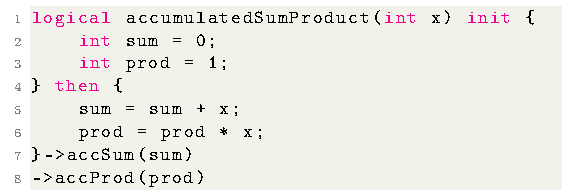
\includegraphics{imgs/functionexamplesimple.pdf}
    \caption{Definition of a Chips function}\label{logical}
\end{figure}

Broadly speaking, when instanciated, a function applies its initializing protocol (the \emph{init} section). Then, it applies its updating process (the \emph{then} section) everytime all its input variables are updated exactly once. If an input variable has a default value, Chips considers it has already been updated once at the initialization of the model. 
Therefore, when connecting input and outputs of functions, one must care about the presence/absence of default values for inputs of components to correctly understand the way dataflow evolve or why some compositions may lead to delayed system deadlock, as shown in figure~\ref{deadlocks}.

\begin{figure}
    \centering
    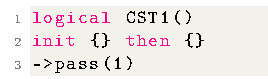
\includegraphics[width=0.3\columnwidth]{imgs/CST1.pdf}
    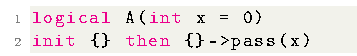
\includegraphics[width=0.3\columnwidth]{imgs/A.pdf}
    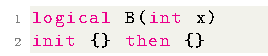
\includegraphics[width=0.3\columnwidth]{imgs/B.pdf}
    \includegraphics[width=\columnwidth]{imgs/Chips_deadlocks.pdf}
    \caption{Presence or absence of deadlocks for sets of functions defined with or without default values for their input.}\label{deadlocks}
\end{figure}

From the model composition perspective, they can be seen as black boxes providing an interface being their set of inputs and their set of outputs. A functional block with all its inputs having a default value is able to \emph{trigger} the components depending on it once because it has all the required information to compute its \emph{then} section once. Remark that functional blocks with no input parameter are always able to compute the content of their \emph{then} section because such computation does not depend on pre-computed data. So they never can be a source of deadlock for the system. 

The composition of functional blocks leads to the creation of a directed graph, which we will call the \emph{functional graph}. The vertices are the functions and the edges are the input/output linkage between the functions. The presence of loops in the graph signifies that at least a part of the designed system retro-acts on itself. Just as the wheels of a vapor train, all functions run their \emph{then} sections altogether, one function giving the pace for the next ones. Therefore, no clock is explicitly defined for the systems. The execution of the \emph{then} section of any component can serve as an implicit clock tick.

The graph formalism applied to the functional dependency of the model elements allow to perform early checking of properties of the model before it is instanciated on a real system.

\subsection{Nodes}

Nodes are an abstraction of the Chips models that represent locations. If two events happen in different places, a model accounting such difference will make each event interact with different nodes. In the context of complex CPSs, nodes can be instanciated to represent a physical separation of processes, or a logical separation for processes that are based on distinct sets of information. Nonetheless, these two use cases of nodes feature common characteristics:
\begin{itemize}
    \item they are responsible of data related to the location they represent, and
    \item they provide a set of typed labels to specify their possibility to exchange data with other nodes.
\end{itemize}

In the case of a node modeling a virtual location, that node is defined as a Chips \emph{object}. An object definition simply gets described as a set of instructions comprising the declaration of \emph{contextual variables} (using the keyword ``ctx'' as in line 3 of Figure~\ref{object}) and the declaration of \emph{channels} (by writing an instruction of two identifiers as in line 4 and 5). Imperative code instructions can also be used in such definitions to define default values of contextual values, but such details go beyond the scope of the system level coordination mechanisms studied in this document.  

\begin{figure}
    \centering
    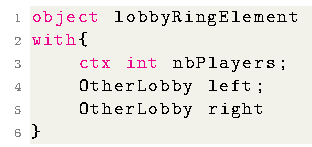
\includegraphics[width=0.5\columnwidth]{imgs/lobbyring.pdf}
    \caption{An object (virtual location) representing an instance of a lobby for a multiplayer server model}\label{object}
\end{figure}

Chips functions can be \emph{embedded} in nodes. When it is the case, functions can refer to contextual variables as if they were defined in their own scope. To do so, we use the \verb'ctx.<ctx_variable_name>' notation in the code sections of the components using it.

Channels are the Chips way to specify how different nodes are connectable together. They feature a \emph{channel type} being an arbitrarily named type (excluding Chips keywords). During the evaluation of the system description section, these channel types allow to ensure the components connected together are compatible.

The definition of a node is orthogonal to the definition of a function, therefore, Chips provides the mean to define functions that are inherently attached to a node. Such concept is particularly relevant when designing components that emulate the physical behavior of a device. This is why such components are defined with the keyword \emph{physical}. The \emph{object} keyword allows to design a node as an abstraction for regrouping functions under a single component with shared contextual values. Such objects cannot exist on their own, they must be instanciated as embedded by physical nodes of a Chips model.

This embedding concept gives rise to a second kind of directed graph, adjacent to the \emph{functional graph} of the previous section. We will call this graph the \emph{mapping graph}. Its vertices can either be functions or nodes, and the edges represent the belonging of a function or a node to another node. Such graph has to be acyclic as an object cannot embed itself.

The graph formalism applied to the concept of embedding allows, just like for the functional graph, to perform early checking of properties of a system, but also to construct upon it the last specificity of Chips, \emph{collective primitives}.

\subsection{Collective primitives}

With the current set of model elements described for Chips, it is possible to define two things:
\begin{itemize}
    \item the evolution of signals among components of a system and
    \item the embedding relation of processes with the parts of system that contain them.
\end{itemize}

However, when designing large systems, the declination of the signals when they have to be spread among many component can become hard, in particular when accounting local information. The current tools available would require to either duplicate our functional blocks as many times as there are different configurations for receiving the data. The same problem is true when it comes to aggregating signals.

Our proposition with the Chips language is to let the programmer design a new kind of operator to describe the way data is modified by the context in which it is spread or collected. Hence the concepts of \emph{spread} and \emph{collect} collective function definitions.

They are comparable to the idea of \emph{Streams} in the java language, except that, instead of processing the evolution of an accumulated value across logical time, they process the evolution of an accumulated value across logical space (i.e.~the stream is updated when it reaches a new components). Such operation is sensitive to the architecture of the model formed, so it cares about the path data takes to go from one node to another. Since the interconnection between nodes is specified by plugging node \emph{channels} together, collective functions also make use of the channels defined to specify data propagation.

A collective function definition is composed of:
\begin{itemize}
    \item a direction keyword (\emph{spread} or \emph{collect}),
    \item a default accumulator definition,
    \item a support node reference,
    \item a stream update code section,
    \item a \emph{target} output expression,
    \item a specification of updated accumulator for each channel of the referenced node.
\end{itemize}

The direction \emph{spread} signify that information transmitted originates from a single component and gets propagated to many others. The direction \emph{collect} signify the information originates from many components and get merged together to become the input of a single one.
The default accumulator definition respects the same rules of the regular Chips function input parameters definition, except that each variable declared as a parameter \textbf{must} be provided with a default value.

To reference a support node, simply use the name of the node definition to use as support. This allows to compute when the stream update process is relevant to apply, thus respecting the \emph{mapping graph} for the propagation of data.

The target output expression must be of the type of the input of the Chips function that will receive the propagated data. It is annoted with the \texttt{@} symbol.

Updated accumulators must be specified for each channel that is defined for the type of node that the collective function references.
\begin{itemize}
    \item For \emph{spread} operations, all of the channel accumulators but the one that provided the input accumulator to the collective function will be used.
    \item For \emph{collect} operations, only the channel accumulator that goes in the direction of the collecting component will be used.
\end{itemize}

Chips provides a \emph{default} accumulator keyword to define the updated accumulator expression for all the channels that do not have a specification yet.
In the context of collective functions, the set of instructions for the stream update code section is the same as the one from regular functions. However, the semantics of expressions in this context differs in two different ways:
\begin{itemize}
    \item each datatype is enhanced with a new value (represented by the keyword \emph{stop})
    \item some new variables are available by default (the \emph{input} and channel related and variables).
\end{itemize}

\subsubsection{Semantics for \emph{stop}}
The \emph{stop} value is to signify that a variable must not be processed anymore during a collective operation. 
\paragraph{During a spread operation} Any component receiving a \emph{stop} signal will propagate the stop signal to warn other connected components that they must keep processing information without waiting for a ``fresh'' value. 
\paragraph{During a collect operation} Any component receiving a \emph{stop} signal will assume the collect operation must be completed using the defaut accumulator instead of a pre-computed one.
The \emph{stop} keyword can be used as a value of any primitive type during the implementation of the code section of a collective primitive. Any operation applied to a \emph{stop} operand will result in the \emph{stop} value.

\subsubsection{Defaultly available variables}

\paragraph{input} is the read-only variable representing the value provided by the Chips function that is the source of the data spread/collected. In the context of a \emph{spread} collective function, it should appear in expressions of the default accumulator definition only. In the context of a \emph{collect} collective function, it should appear in expressions of the stream update code section and/or the updated accumulators expressions. A collective function \textbf{must} feature at least one occurence of the \emph{input} variable.

\paragraph{channel related variables} are a way to refer to accumulators when they are provided through a specific channel of the node. These variables are read-only and can be accessed with the notation
\begin{center}
    \verb'<channel_name>.<accumulator_parameter_name>'
\end{center}
within any expression of the correct type. In case the data read hasn't been initialized because no component is connected through the given channel or because the data transmitted contained a \emph{stop} value, the values of the parameters for that channel are the default values defined for the accumulator of this collective function definition.

Figure~\ref{collectexample} presents an example of definition for a collective function featuring all the metionned characteristics above. This example is pretty absurdly complicated for the sake of demonstrating all the usable features of collective function definitions. For this example to be fully functional, we assume that contextual values are previously set by other Chips functions linked to each instance of \emph{ContainerObject}. We also assume the objects are correctly connected together by associating each channel of a given \emph{ContainerObject} to at most one channel of another \emph{ContainerObject}.

It is worth noting that for each channeled accumulator defined, the types of the provided expression respect the types of the default accumulator. If it hasn't been the case, an error would have been raised.
\begin{figure}
    \centering
    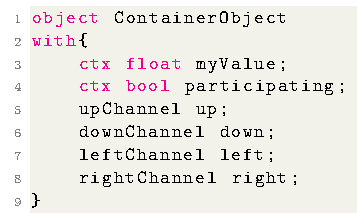
\includegraphics[width=0.3\columnwidth]{imgs/ContainerObject.pdf}
    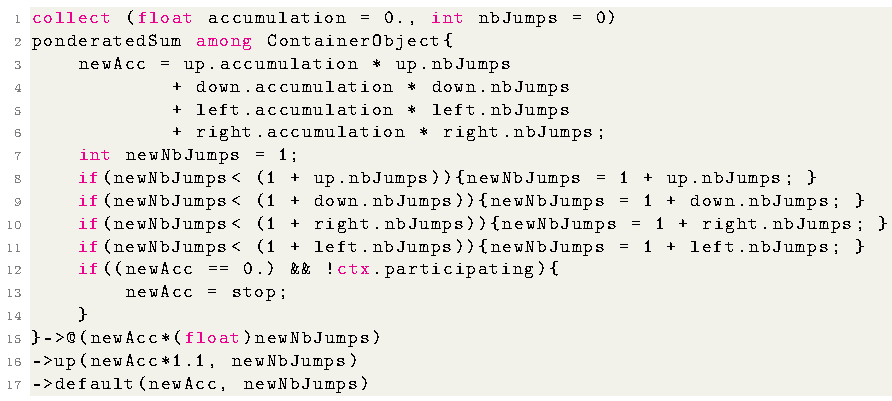
\includegraphics[width=0.65\columnwidth]{imgs/collectivefunctionexample.pdf}
    \caption{An object definition and a collective function to compute a sum of all the functions among the defined object, ponderated by the longest path to a leaf of the tree formed by the configuration used to collect data, putting an emphasis on data propagated via the \emph{up} channel.}\label{collectexample}
\end{figure}

\newpage
\section{Formalisation of Chips modeling semantics}\label{osemantic}

This section is dedicated to mathematically describe the elements of the Chips language that were described earlier in a less formal way. At first, we will define the formalism related the language \emph{functional graphs} (graphs related to the functional block dependencies). Secondly, we will put our focus on the \emph{mapping graphs} (graphs related to the association of functions and virtual objects to physical devices). Finally, we will see how the interconnections between virtual and physical objects define the structures of the datastreams that are spread and collected among a system when using Chips collective primitives.

\subsection{On functional graphs}

The concept of functional graph can be directly derived from the idea that, for a component system to work, it realizes simultaneously all the processes that it is built for. It makes use of coordination techniques to synchronize processes that depend on each others. Each process implemented is, within functional graphs, a vertex, while each synchronization of two processes is an edge. On systems where waiting delays are short enough to be ignored, the synchronous paradigm becomes a powerful tool to analyze, predict or design such systems. Thus, many languages of that sort have emerged for a wide variety of use cases (embedded systems, safety-critical systems, multi-physics modeling, FPGA programming\dots)\cite{halbwachs_synchronous_2005,leguernic_programming_1991,bourke_zelus_2013,dragoi_psync_2016,sylvestre_programmation_2024}. Chips specificity lies in its ambition to model and control cyber-physical systems where components can be composed hierarchically, in a distributed manner and with run-time reconfiguration faculties. With that in mind, its operational semantics must include a number of features that we will detail here before achieving the graph-like structure for processes interconnection that is characteristic to synchronous languages.


\Notation{Tuple usage} In the rest of this document, for any given tuple $t = (t_1, t_2, \dots)$, we will write $t.t_1, t.t_2, \dots$ to reference the elements that compose $t$.

\newcommand{\I}{\mathbb{I}}
\renewcommand{\O}{\mathbb{O}}
\newcommand{\X}{\mathbb{X}}
\renewcommand{\S}{\mathbb{S}}
\renewcommand{\F}{\mathbb{F}}

\Notation{Inputs, outputs, variables and expressions} From now on, we will denote respectively $\I$, $\O$ and $\X$ the sets of correctly typed inputs, outputs and variables for Chips functions across the scope of any system description. $\S$ will refer to the set of all correct string sequences for names of variables, inputs, outputs and functions. Any $i \in \I$ is a tuple of the form $i = (name, value)$, any $o \in \O$ is a tuple of the form $o = (name, exp)$, Any $x \in \X$ is a tuple of the form $x = (name, value)$ with:
    \begin{itemize}
        \item names $\in \S$ being all chosen pair-wise distincts across $\I$, $\O$ and $\X$, unless specified,
        \item values and expressions being tuples featuring an attribute $t$, their respective type.
    \end{itemize}
    We will assume values and expressions are correctly composed and typed within Chips instructions and expressions.

\begin{remark}
    Since Chips is \emph{partially}-synchronous, some specific code sections\footnote{The code sections dedicated to defining components inner variables and their updating procedures} are to be written using an imperative syntax. In these sections, Chips defines instructions and expressions in a way that is similar to other imperative languages. For concision purposes, we will not detail their semantics and refer to~\cite{plotkin_structural_1981} for examples of equivalent formal interpretation. For the same reasons, no further detail either will be given on the data structures used to represent values.
\end{remark}

Functional graphs use functions as primary components.

\begin{definition}\label{functional_block}
    A correctly defined Chips \emph{functional block}, belonging to a set we will call $\F$, is a tuple\\$f = (B, I, O, I_{default},X_L, X_{init}, then, ready)$, where:
    \begin{itemize}
        \item $I \subset \mathbb{I}$ and $O\subset\mathbb{O}$ are finite;
        \item $I_{default} \subset \mathbb{I}$ is the (potentially empty) set of default values for the inputs of $f$ when they are provided;
        \item $ready$ is a boolean variable set to:
        \begin{equation*}
            ready = (start \wedge (\forall i \in I, \exists i_{default} \in I_{default}, i.name = i_{default}.name)),
        \end{equation*} 
        with $start$ is arbitrarily set to $\top$ or $\bot$;
        \item $X_L \subset \X$ is a finite set of local variables;
        \item $X_{init} \subset \X$ corresponds to the initial value of $X_L$ (defined by a process that we will abstract here),
        \item $then \in 2^{I \times X_L \mapsto X_L \times O}$ is singleton containing the process that modifies the values of $X_L$ and/or $O$ according to the values of $I$ and the past values of $X_L$\footnote{$f.then$ refers to a set of processes instead of directly to a process to have an easier compatibility with the formalism of the composition of functional blocks, which is the subject of further definition~\ref{composition}};
        \item $B$ is a non-deterministic Labelled Transition System (LTS) that models the behavior of the function. It must be defined according to the nextly presented defintion.
    \end{itemize}
\end{definition}

\Notation{Updating process} For a given functional block $f \in \F$, we will write directly $f.\pi$ to refer to the only element contained by $f.then$.  

\begin{definition}\label{functional_block_behavior}
    Let $f\in\F$ be a functional block. Its \emph{behavior} $f.B$ is specified as a LTS. Classically, we define it as a tuple $ f.B = (Q, \Sigma, \Delta, q_0, q_f)$, where:
    \begin{itemize}
        \item $Q$ is the set of states of our LTS;
        \item $q_0$ and $q_f$ are respectively the LTS initial and final states;
        \item $\Sigma = \{x.name~|~x \in I \cup O\}\cup \{\varepsilon, init\}$ serves as the alphabet/list of labels of our LTS. $\varepsilon$ classically used for the $\varepsilon$-transitions of non-deterministic automata, and $init$ represents a setting-up event for the function;
        \item $\Delta$ is the set of all the transition relations of the form $\delta = (q, event, guard, q') \in Q \times \Sigma \times \{\top,\bot\} \times Q$ that are associated to $f$.
    \end{itemize}
    Of course, not all LTS fit as a functional block behavior. A correct behavior for $f$ contains exactly $2^{\#f.I} + 2^{\#f.O}$ states:
    \begin{itemize}
        \item 2 states representing the initial state $q_{init}$ and the idle state $q_{\emptyset}$,
        \item $2^{\#f.I}-1$ states, each labelled by a different \textbf{non-empty} (hence the ``$-1$'') unordered set $\iota=\{i.name~|~i\in I'\subseteq f.I\}$, which we will write $q_\iota$ for short,
        \item $2^{\#f.O}-1$ states, each labelled by a different \textbf{non-empty} unordered set $\omega=\{o.name~|~o\in O'\subseteq O\}$, which we will write $q_\omega$ for short.
    \end{itemize}
    From these states, we have $f.q_f = q_{\emptyset}$ and naturally, $f.q_0 = q_{init}$. The transition relation is then built according to $f$. A transition $\delta = (q, event, guard, q')$ belongs to $f.\Delta$ if and only if all the following assertions are true:
    \begin{multline}
        (\delta.q, \delta.q')\in \{(q_I,q_O), (q_{init},f.q_I), (q_{init}, q_\emptyset)\}\\
        \cup \{(q_{\iota},q_{\iota'})~|~\iota\subset\iota' \wedge (\#\iota = \#\iota'-1)\}\\
        \cup \{(q_{\omega},q_{\omega'})~|~\omega\supset\omega' \wedge (\#\omega' = \#\omega-1)\}
    \end{multline}
    \begin{equation}
        \begin{split}
        (\delta.q = q_{init} \Leftrightarrow \delta.event = init)\s\wedge\s(\delta.q = q_{I} \Leftrightarrow \delta.event = \varepsilon)\s\s\s\\
        \wedge (\forall \iota \subset I, \forall x \in I, (q, q') = (q_{\iota},q_{\iota\cup\{x.name\}}) \Leftrightarrow \delta.event = x.name)\s\halfs\\
        \wedge (\forall \omega \subset O, \forall x \in O, (q, q') = (q_{\omega\cup\{x.name\}},q_{\omega}) \Leftrightarrow \delta.event = x.name)
        \end{split}
    \end{equation}
    \begin{equation}
        guard \Leftrightarrow [(q \neq q_{init}) \vee (f.ready \wedge (q' = q_I)) \vee (\neg f.ready \wedge (q' = q_\emptyset))]
    \end{equation}
\end{definition}

\Notation{Assignment and substitution} In the remaining of this document, informally, we will write $A := B$ to mean ``$A$ is assigned the value of $B$'', and $A[B := C]$ to mean ``the value $A$ for which, in its definition, every instance of the value $B$ gets assigned the value $C$ instead''.

\Notation{Transitions on LTSs} For a given transition of the form 
\begin{equation*}
    \delta = (q, event, guard, q') \in LTS
\end{equation*}
we use the syntax $q\aoverb{\delta}{\rightarrow}q'$ as a shorthand when $\delta.guard = \top$.

\begin{definition}
    Let $f = (B, I, O, I_{default},X_L, X_{init}, then ready)$ be a correctly defined functional block. The \emph{operational semantics} of $f$ is given by an LTS $\sigma(f) = (Q,\Sigma, \rightarrow)$, using $q \in f.Q$ as the control state, and $\rightarrow$ being the minimal transition relation inductively defined by the rule:
    \begin{equation}
        \centering
        \begin{split}
            q = \delta.q \s\s evt = \delta.event\s\s q' = \delta.q'\s\s\s\\
            \cfrac{
                \s\s q\aoverb{\delta}{\longrightarrow}q' \s\s(I,X_L,O) := \pi_{q,q'}(I,X_L,O)\s\s
            }
            {
                q \aoverb{evt}{\longrightarrow} q'
            }
        \end{split}
    \end{equation}
    where $\pi_{q,q'} : I \times X_L \times O \mapsto I \times X_L \times O$ is the process to interpret whenever a transition is applied from state $q$ to state $q'$. Let ``$;$'' be the sequence evaluation operator and $nop$ be the empty process in the following definition:
    \begin{equation*}
        \pi_{q,q'}:
        \begin{cases}
            \text{ if } q = q_{init} & \text{ then } X_L:= X_{init}; \pi_{init}\\
            \text{ if } (q,q') = (q_{I}, q_{O}) & \text{ then } (X_L, O) := f.\pi(I,X_L)\\
            & \text{ otherwise } nop\\
        \end{cases}
    \end{equation*}
    where
    \begin{equation*}
        \pi_{init} \eqdef I := I[\{ i~|~name(i) \in names(I_{default}) \} := I_{default}].
    \end{equation*}
\end{definition}

Now that functions and their behavior are defined, the last elements needed before assembling functions into our functional graphs are the dataflows which let functional blocks ``feed'' each other.

\begin{definition} 
    Let $F\subset \F$ be a finite set of functional blocks. A \emph{dataflow} is a tuple $d=(source,sink,value,B)$, where:
    \begin{itemize}
        \item $source\in\bigcup_{f \in F} f.O$,
        \item $sink\in\bigcup_{f \in F} f.I$,
        \item $value$ is a Chips data that is transmitted through the dataflow,
        \item $source.type = sink.type = value.type$ and
        \item $B = (Q, \Sigma, \Delta, q_0, q_f)$ is a LTS explicitly defined by:
        \begin{itemize}
            \item $Q = \{q_{rcv}, q_{snd}\}$ as the set of states,
            \item $\Sigma = \{source.name, sink.name\}$ as the alphabet,
            \item $\Delta = \{(q_{rcv},source.name,\top,q_{snd}), (q_{snd},sink.name,\top,q_{rcv})\}$ as the set of transition relations,
            \item $q_0 = q_{rcv}$ as the initial state and
            \item $q_f = q_{snd}$ as the final state. 
        \end{itemize}
    \end{itemize}
\end{definition}

\begin{definition} 
    Let $d\in F[\F]$, a dataflow. Its \emph{operational semantics} is given by $d.B$, applying either of these rule when using its transitions:
    \begin{equation}
        \cfrac{
            \delta.event = d.source.name \s\s\s d.value := d.source.value
        }
        {
            q_{rcv} \aoverb{\delta}{\longrightarrow} q_{snd}
        }
    \end{equation}
    \begin{equation}
        \cfrac{
            \delta.event = d.sink.name \s\s\s d.sink.value := d.value
        }
        {
            q_{snd} \aoverb{\delta}{\longrightarrow} q_{rcv}
        }
    \end{equation}
    \noteag{I feel like I wrote something wrong but I don't see what\dots}
\end{definition}

\Notation{Dataflow set} A dataflow is a data structure that is tied to a set of functional blocks. For a given finite set of functional blocks $F \subset \F$, we write $D[F]$ the set of all the dataflows over $F$.

\begin{definition} 
    \emph{Functional graphs} are, as described in Section~\ref{functions}, a finite directed graph $G_F = (F,D)$ for which vertices $F\subset\F$ (for functions) are instances of functional blocks and edges $D \subset D[F]$ (for dataflows) are the input/output relations between such blocks.
    A functional graph $G_F$ holds the following properties:

    \begin{equation}\label{input_completeness}
        \text{(input completeness)}\s\s\s\s\halfs\forall f\in F,\forall i \in f.I, \exists d \in D, i = d.sink\s\s\s\halfs
    \end{equation}
    \begin{equation}\label{output_completeness}
        \text{(output completeness)}\s\s\s\s\forall f\in F,\forall o \in f.O, \exists d \in D, o = d.source\s\s
    \end{equation}
    \begin{multline}\label{sources_unicity}
        \text{(dataflow sources unicity)}\s\s\forall f\in F, \forall o \in f.O,\\
        [(\exists d_1 \in D, d_1.source = o)\wedge(\exists d_2 \in D, d_2.source = o)] \Rightarrow (d_1 = d_2)
    \end{multline}
    \begin{multline}\label{sinks_unicity}
        \text{(dataflow sinks unicity)}\s\s\forall f\in F, \forall i \in f.I, \\
        [(\exists d_1 \in D, d_1.sink = i)\wedge(\exists d_2 \in D, d_2.sink = i)] \Rightarrow (d1 = d2)
    \end{multline}
\end{definition}

\Notation{Functional graphs acronyms} For short from now on, we will write \emph{DIOC} for Dataflow Input/Output Completeness and \emph{DSSU} for Dataflow Sources and Sinks Unicity. 

With these defintions, the semantics of functional blocks can now be extended as the semantics of a \emph{composition} of functional blocks. In a given functional graph $G_F = (F,D)$, all functional blocks of $F$ are to be executed in parallel. Therefore, the operational semantics of each functional block has to stand simultaneously. However, the input/output dependecy of functions, modeled by dataflows, imply the synchronization of the different automata of a system. Thus, the need to define a composition operation.

\begin{definition}\label{composition}
    Let $f_1,f_2 \in\F$ two distinct functional blocks. We define the parallel composition operation of $f_1$ and $f_2$ relatively to a dataflow $d \in~D[\F]$ as:
    \begin{align}
        f_1 ||_d f_2 = (B, I, O, I_{default}, X_L, X_{init}, then, ready)
    \end{align}
    where: 
    \begin{itemize}
        \item $B = f_1.B \mprod d.B \mprod f_2.B$, $\mprod$ being the mixed (or synchronous) product as defined in~\cite{duboc_mixed_1986},
        \item $I = f_1.I\cup f_2.I -\{d.sink\}$,
        \item $O = f_1.O\cup f_2.O -\{d.source\}$,
        \item $I_{default} = f_1.I_{default}\cup f_2.I_{default}$,
        \item $X_L = f_1.X_L \cup f_2.X_L$,
        \item $X_{init} = f_1.X_{init} \cup f_2.X_{init}$,
        \item $then = f_1.then \cup f_2.then$, and
        \item $ready = f_1.ready \wedge f_2.ready$
    \end{itemize}
    To compose a functional block $f_1$ with itself relatively to a dataflow $d \in~D[\F]$, we will also write it as:
    \begin{align}
        f_1 ||_d f_1 = (B, I, O, I_{default}, X_L, X_{init}, then, ready)
    \end{align}
    but instead we will have:
    \begin{itemize}
        \item $B = f_1.B \mprod d.B$,
        \item $I = f_1.I -\{d.sink\}$,
        \item $O = f_1.O -\{d.source\}$,
        \item $I_{default} = f_1.I_{default}$,
        \item $X_L = f_1.X_L$,
        \item $X_{init} = f_1.X_{init}$,
        \item $then = f_1.then$, and
        \item $ready = f_1.ready$
    \end{itemize}
\end{definition}

\Notation{Set of complex functional blocks} Until then, we used $\F$ as the set of correctly defined functional blocks. With composition, this set can be expanded to the set of complex functional blocks which we will call $\F^*$, such that, $\F \subset \F^*$ and for any $d\in D[\F]$, $\F^*$ is closed by the parallel composition operation relatively to $d$. Thus, $||_d$ is an internal composition law of $\F^*$


\begin{remark}
    About associativity, as claimed by C. Duboc in~\cite{duboc_mixed_1986}, definition 2.3, the mixed product $\mprod$ is associative. Since all other operations used to define the elements of the parallel composition are associative, we assume the parallel composition is associative.
    
    % when defining our system functional blocks, all the names used are chosen pair-wise distincts accross functions, parameters and variables. Therefore, for any pair made of a functional block and a dataflow $(f,d)\in \F\times D[\F]$, if $d$ doesn't reference any element of $f.I$ or $f.O$, there is no name collision on the labels of $f.B$ and $d.B$, which renders their mixed product isomorphic to the direct product of $f.B$ and $d.B$. The same is true for any $(d,f)\in D[\F] \times \F$. \noteag{I don't know how to say it :')} 
\end{remark}

\begin{remark}
    About commutativity, the mixed product isn't strictly commutative, for any two elements $f_1,f_2 \in \F^*$, states of $(f_1 ||_d f_2).B$ are in $f_1.B.Q \times f_2.B.Q$ and states of $(f_2 ||_d f_1).B$ are in $f_2.B.Q \times f_1.B.Q$. However, $f_1 ||_d f_2$ is isomorphic to $f_2 ||_d f_1$.
    It is reasonable to assume that there always exist a total order $\preccurlyeq$ over the elements of any finite subset of $\F$.
    Let such order be used. For the rest of this paper, we will consider a tweaked version of the mixed product where each state $(q_\alpha,q_\beta) \in A \times B$ is renamed as $q_{sort(\alpha\cup\beta)} \in 2^{A\cup B}$. Such renewed mixed product is now commutative, and so becomes our parallel composition operation.
\end{remark}

\begin{definition}
    Let $f_i = (B_i, I_i, O_i, {I_{default}}_i, {X_L}_i, {X_{init}}_i, then_i, ready_i)$, for $i = 1,2$ be two elements of $\F^*$ each being either an atomic functional block or a composition of functional blocks, let $d = (source_d,sink_d,value_d,B_d) \in D[\F]$. The \emph{operational semantics} of $f_1 ||_d f_2$ is a LTS $\sigma(f_1 ||_d f_2) = (Q,\Sigma, \rightarrow)$, using $(q_1,q_d,q_2) \in f_1.B.Q \times d.B.Q \times f_2.B.Q$ as the control state, $\Sigma = f_1.B.\Sigma \cup d.B.\Sigma \cup f_2.B.\Sigma$ and $\rightarrow$ being the minimal transition relation inductively defined by the rules:

    \begin{equation}
        \cfrac{
            \exists \delta \in B_1.\Delta, \nexists \delta' \in B_d.\Delta, \delta.event = a \wedge \delta'.event = a, q_1\aoverb{\delta}{\longrightarrow}q_1'
        }
        {
            q_1,q_d,q_2 \aoverb{a}{\s\longrightarrow\s} q_1',q_d,q_2
        }
    \end{equation}

    \begin{equation}
        \cfrac{
            \exists \delta \in B_1.\Delta, \exists \delta' \in B_d.\Delta, \delta.event = a = \delta'.event, q_1\aoverb{\delta}{\longrightarrow}q_1',q_d\aoverb{\delta'}{\longrightarrow}q_d' 
        }
        {
            q_1,q_d,q_2 \aoverb{a}{\s\longrightarrow\s} q_1',q_d',q_2
        }
    \end{equation}

    \begin{equation}
        \cfrac{
            \exists \delta \in B_2.\Delta, \nexists \delta' \in B_d.\Delta, \delta.event = a \wedge \delta'.event = a, q_2\aoverb{\delta}{\longrightarrow}q_2'
        }
        {
            q_1,q_d,q_2 \aoverb{a}{\s\longrightarrow\s} q_1,q_d,q_2'
        }
    \end{equation}

    \begin{equation}
        \cfrac{
            \exists \delta \in B_2.\Delta, \exists \delta' \in B_d.\Delta, \delta.event = a = \delta'.event, q_2\aoverb{\delta}{\longrightarrow}q_2',q_d\aoverb{\delta'}{\longrightarrow}q_d' 
        }
        {
            q_1,q_d,q_2 \aoverb{a}{\s\longrightarrow\s} q_1,q_d',q_2'
        }
    \end{equation}
    where $a$ is an element of $B_1.\Sigma \cup B_d.\Sigma \cup B_2.\Sigma$.
\end{definition}

\begin{definition}
    Let $G_F = (F, D)$ a correcly defined functional graph ensuring DIOC and DSSU. The \emph{operational semantics} of such functional graph $\sigma(G_F)$ is given by the successive parallel composition of all the functional blocks of $F$ relatively to all the dataflows of $D$.
\end{definition}


\myrule
Everything below this comment is TODO.
\myrule
\subsubsection{Properties of Chips functional graphs}

In this (subsub)section, we must define:
\begin{itemize}
    \item proof of deadlock freedom for complete graphs with DSS unicity ? 
    \item feedback mechanisms (cyclic graphs)
    \item implicit logical clock cycles description
\end{itemize}

\subsection{On mapping graphs}

In this (sub)section, we must:
\begin{itemize}
    \item formalize the definition for mapping graphs
    \item list important properties of such graphs 
\end{itemize}

\subsubsection{Definitions over mapping graphs}

In this (subsub)section, we must define:
\begin{itemize}
    \item node channels
    \item node contextual data
    \item node types: physical and objects
    \item linking (embedding) functions to nodes
    \item linking (embedding) objects to physicals
    \item plugging channels together
\end{itemize}


\subsubsection{Properties of Chips mapping graphs}

In this (subsub)section, we must define:
\begin{itemize}
    \item configurations (embedding DAGs)
    \item functional graph mapping: check if a configuration can support a logical synchronous program
    \item envisionned properties for model checking (reconfigurability, timing robustness, imprecision robustness, others\ldots?)
\end{itemize}

\subsection{On collective primitives}

In this (sub)section, we must:
\begin{itemize}
    \item formalize the definition for spread and collect
    \item list properties enabled by this concept 
\end{itemize}

\subsubsection{Formal definitions for collective primitives}

In this (subsub)section, we must define:
\begin{itemize}
    \item relation with functional graph (safe breaking of DSS unicity)
    \item relation with mapping graph (more particularly nodes and the concept of configuration)
\end{itemize}


\subsubsection{Properties enabled by collective primitives}

In this (subsub)section, we must define:
\begin{itemize}
    \item implementation of control motifs
    \item sensitivity/robustness to reconfigurations
\end{itemize}

\section{Current Chips implementation}
Must talk about:
\begin{itemize}
    \item compilation pipeline
    \item example implemented
\end{itemize}


\section{Current, Future and Related Works}

\subsection{Current and future}

Must talk about:
\begin{itemize}
    \item custom data structures
    \item specification files for domain specific property checking
    \item example implemented for JavaBIP
    \item embeddable code generation
    \item reconfiguration specifications
\end{itemize}

\subsection{Related}
Maybe it should be placed somewhere else in the paper if it is a paper.

Must talk about:
\begin{itemize}
    \item Lustre, Esterel, Signal, Fiacre, VHDL, Amaranth, Eclat, ScaFi, BIP, Tina, Hippo
    \item GenoM specifications for hierarchical models
\end{itemize}


\section{Conclusion}

On a vraiment fait du bon travail, c'est super!

\printbibliography

\end{document}